\documentclass[11pt,a4paper]{article}
\usepackage[utf8]{inputenc}
\usepackage[T1]{fontenc}
\usepackage{lmodern}
\usepackage{upgreek}
\usepackage[slovene]{babel}
\usepackage{color}
\usepackage{graphicx}
\usepackage{verbatim}
\usepackage{amsmath}
\usepackage{float}
\usepackage{xcolor}
\usepackage{todonotes}
\usepackage{listings}
\usepackage{xparse}
\usepackage{icomma}
\usepackage[backend=bibtex]{biblatex}
\addbibresource{viri.bib}
\usepackage[title]{appendix}

% code styling
\lstset{language=Python,keywordstyle={\bfseries \color{blue}}}
\NewDocumentCommand{\codeword}{v}{%
	\texttt{\textcolor{blue}{#1}}%
}
\DeclareMathOperator{\Hz}{Hz}
\DeclareMathOperator{\kHz}{kHz}

\begin{document}

\title{Nadgradnja sistema za merjenje koncentracije trdnih delcev v zraku s tipalom Sharp GP2Y1010AU0F}
\author{"Ziga Pata"cko Koderman \and Klemen Bu"car}
\date{\today}

\clearpage\maketitle
\thispagestyle{empty}
\pagebreak

\tableofcontents
\pagebreak

\section{Uvod}
\todo{prvo stran moram "se dokoncati}
\todo{vsem grafom moram dodati enote in jih spremeniti v pdf}

Cilj projekta je razviti cenovno ugoden sistem za opravljanje meritev koncentracije trdnih delcev v zraku ter oceniti njegovo negotovost. Za ta namen je bilo izbrano tipalo GP2Y1010AU0F podjetja Sharp \cite{sharp-gp2y1010au0f}. To je opti"cni senzor, ki za delovanje izkori"s"ca odvisnost med koli"cino sipane svetlobe pri potovanju skozi medij in koncentracijo delcev.

\todo{Izbran je bil ta in ta senzor zato in zato...}
\todo{vec teksta, kaj vse je poleg senzorja bilo uporabljeno}
\todo{ena slikca setupa}
\todo{kaj je bilo ze, kaj je moj del}

\pagebreak

\section{Obstoje"ca konfiguracija}

Tipalo Sharp GP2Y1010AU0F \cite{sharp-gp2y1010au0f} sestavljata infrarde"ca LED, ki v pulzih emitira IR svetlobo, ter fototranzistor za detekcijo sipane svetlobe. Oba sta zaprta v ohi"sje in postavljena v kota ob isti stranici tako, da svetloba iz diode ne prehaja neposredno na fototranzistor (slika \ref{sensor-scheme}). Meritev opravimo tako, da LED vklopimo s kratkim pulzom preko RC vezja ter opazujemo odziv fototranzistorja, ki je posledica:
\begin{itemize}
	\item odboja svetlobe od notranjih sten ohi"sja in
	\item sipanja svetlobe pri potovanju skozi medij.
\end{itemize}

\begin{figure}[H]
	\begin{center}
		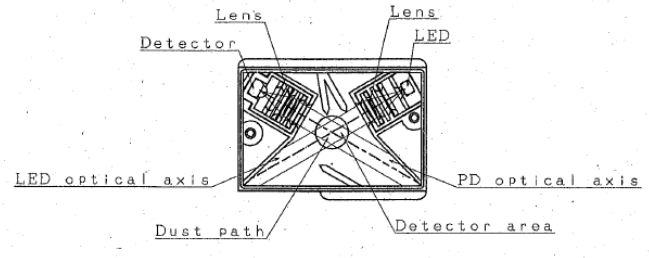
\includegraphics[width=12cm]{sensor-scheme.png}
		\caption{Skica tipala GP2Y1010AU0F}
		\label{sensor-scheme}
	\end{center}
\end{figure}

Proizvajalec tipala priporo"ca, naj za pro"zenje IR LED uporabimo RC vezje z $220\ \mu f $ kondenzatorjem in $150\ \Omega $ uporom \cite{sharp-gp2y1010au0f}. Karakteristi"cni "cas takega vezja je

$$
\uptau = RC = 0,033\ s
$$

Po vsakem pulzu LED moramo vezje spet napolniti, za kar porabimo nekaj karakteristi"cnih "casov. Predpostavimo, da trije karakteristi"cni "casi zadostujejo.

$$
\nu = \frac{1}{t_0} \approx \frac{1}{3 \uptau} = 10\ \Hz
$$

Meritve lahko torej opravljamo s frekvenco najve"c $ 10\ \Hz $. Vsakokrat opazujemo odziv fototranzistorja. To je napetostni impulz, ki ga vzor"cimo z 10-bitnim ADC (ang. \textit{analog to digital}) pretvornikom MCP3002 \cite{mcp3002}, in dobimo njegovo digitalno obliko.

Celoten proces, ki zajema:
\begin{itemize}
	\item krmiljenje infrarde"ce LED,
	\item branje pretvorjenega signala,
	\item komunikacijo z RTC (ang. \textit{real time clock}) modulom in
	\item shranjevanje meritev,
\end{itemize}

krmili mikrora"cunalnik Raspberry Pi \cite{rbpi-wiki}.

\begin{figure}[H]
	\begin{center}
		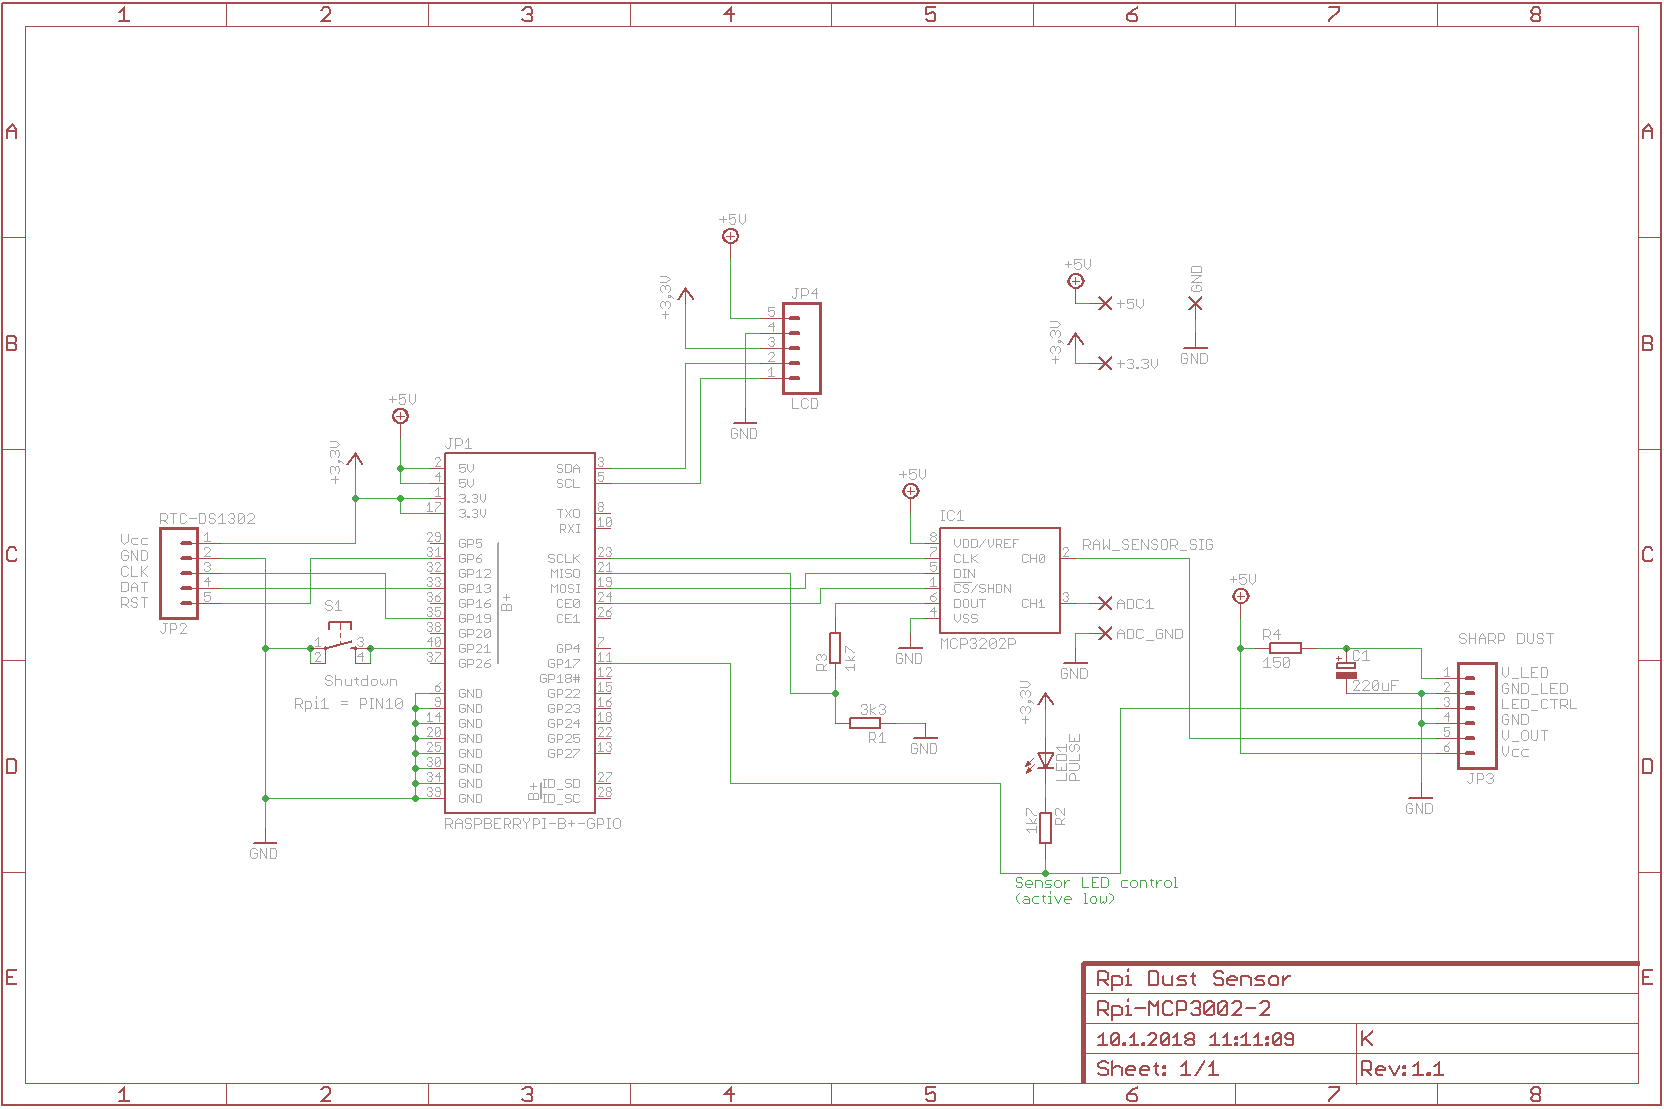
\includegraphics[width=12cm]{scheme.png}
		\caption{Shema vezja}
	\end{center}
\end{figure}

Prebrani pulz vzor"cimo s frekvenco $ \approx 35,7\ \kHz $ (kolikor zmore Raspberry Pi) ter ga shranimo kot mno"zico 50 to"ck, v tabelo znotraj HDF5 datoteke \cite{hdf5}.

Proizvajalec priporo"ca, da napetost na fototranzistorju od"citamo $0,28\ ms$ po vklopu LED. Kljub temu na"s sistem zajema odziv fototranzistorja $ 1,4\ ms $ od vklopa LED. "Cas $0,28\ ms$ sovpada z vrhovi izmerjenih pulzov, tako da predvidevamo, da v resnici i"s"cemo vrh pulza. 

\begin{figure}[H]
	\begin{center}
		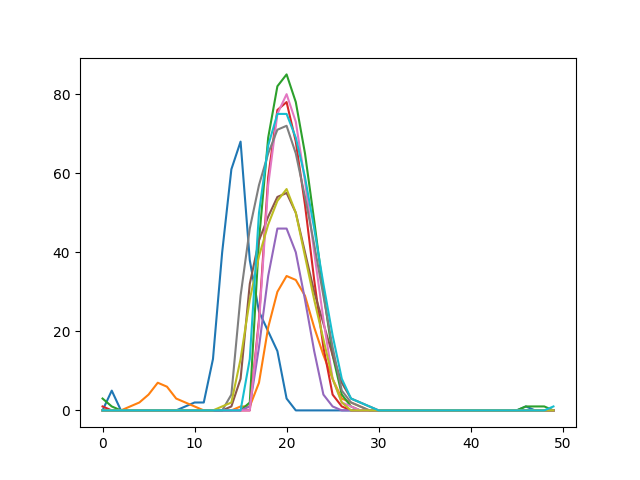
\includegraphics[width=12cm]{pulses_old.png}
		\caption{Primer 10 odzivov fototranzistorja}
		\label{pulses-old}
	\end{center}
\end{figure}

S slike \ref{pulses-old} je razvidno, da vzorci pulzov med seboj niso preve"c podobni. Vrhovi so zelo razpr"seni in odstopajo za $ \approx \pm 40\ \% $.

Meritve primerjamo tudi z meritvami, opravljenimi z referen"cnim tipalom Grimm Mini-LAS 11-R \cite{grimm-min-las}. Korelacijo med vi"sinami izmerjenih vrhov in podatki tipala Grimm opazimo "sele po zelo obse"znem povpre"cenju nekaj 1000 vrhov, "se ta pa ostaja manj"sa od negotovosti meritve.

\clearpage

\section{Nadgradnja}
Zaradi neuporabnosti obstoje"cih meritev se odlo"cimo za sistemati"cno analizo in nadgradnjo obstoje"cega sistema za zajem in analizo vzorcev.

\subsection{Neenakomerno vzor"cenje}
Zaradi variabilne obremenitve procesorja na krmilniku Raspberry Pi dobi proces za zajemanje meritve spremenljivo koli"cino procesorskega "casa. To"ck na pulzu torej ne od"citavamo z enakomerno frekvenco. Odstopanja odpravimo tako, da vsaki to"cki dodamo "casovno "stampiljko \todo{mogoce rajsi oznako?}.

\begin{figure}[H]
	\begin{center}
		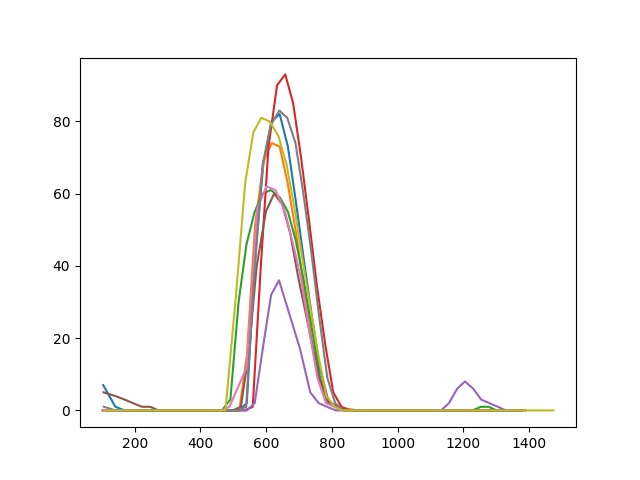
\includegraphics[width=12cm]{aligned.png}
		\caption{Pulzi po "casovni poravnani izmerjenih to"ck}
		\label{aligned}
	\end{center}
\end{figure}

Ko to"cke poravnamo relativno na "cas v"ziga LED, opazimo precej lep"so poravnavo vrhov (slika \ref{aligned}).

\subsection{Velikost vzorca}
Pri opravljanju meritve ne poznamo natan"cnega pretoka zraka skozi tipalo. Zana"samo se na konvekcijsko gibanje zraka. Da preverimo, ali to zadostuje za potrebe meritve, pretok prisilno pove"camo z ventilatorjem ter opazujemo morebitne spremembe. Ne opazimo nobenih sprememb ter sklepamo, da je konvekcijski pretok zraka dovolj"sen.

\subsection{Svetlobne motnje iz okolice}
Ohi"sje tipala je odprto, da lahko skozenj te"ce zrak. To pa fototranzistor v tipalu izpostavi zunanjim svetlobnim virom. Ti lahko na meritve vplivajo v obliki "suma ali sistemati"cne napake (na primer razlika med dnevom in no"cjo). To preverimo s postavitvijo tipala v popolno temo. Opazimo, da so vrhovi pulzov poravnani bistveno bolje (slika \ref{dark}). Meritve od tu naprej opravljamo v temi.

\begin{figure}[H]
	\begin{center}
		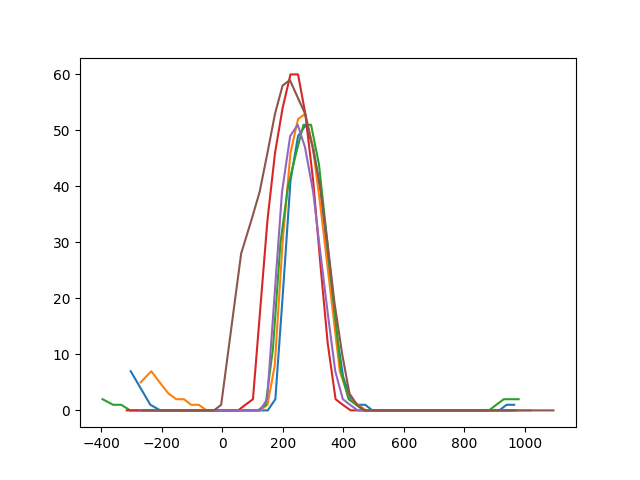
\includegraphics[width=12cm]{dark.png}
		\caption{Pulzi, izmerjeni v temi}
		\label{dark}
	\end{center}
\end{figure}

\subsection{Dolo"canje pravega vrha}
Do zdaj smo pri zajemanju podatkov za vrh pulza vzeli kar najvi"sjo izmerjeno to"cko. Ta pa zaradi premajhne frekvence vzor"cenja nikoli ne sovpada popolnima s pravim vrhom. Napako odpravimo z napenjanjem parabole na najvi"sjih nekaj to"ck. Vsak pulz zajema pribli"zno med 10 in 20 to"ck, tako da se odlo"cimo za napenjanje parabole na najvi"sjih 7.

\subsection{Meritve v vakuumu}
Navkljub vsem izbolj"savam meritve ostajajo polne "suma. Da bi to kvantificirali, postavimo tipalo v vakuum ter popolno temo. S tem "zelimo odstraniti vse zunanje dejavnike ter izmeriti izklju"cno odboj svetlobe od ohi"sja. Napaka meritve v tem primeru prihaja iz negotovosti pri od"citavanju ter neenakomernih pulzov LED.

Razlike med meritvami na prostem in v $ 15mbar $ vakuumu ne zaznamo. Sklepamo, da potrebujemo "se ni"zji pritisk.

\todo{slikca iz vakuuma mogoce?}

\subsection{Nadgradnja analize podatkov}
Analiza podatkov poteka na lo"cenem ra"cunalniku in ni del naprave za opravljanje meritev. Obstoje"ci sistem za obdelavo meritev povpre"ci vi"sine vrhov pulzov v "zelenem "casovnem obdobju (nekaj 10 minut). Rezultate skupaj z meritvami, opravljenimi z merilnikom Grimm mini-LAS, nari"se na graf. Posebne korelacije ne opazimo. Da bi to kvantificirali, korelacijo tudi izra"cunamo  \todo{manka vir iz knjige k je na IJS-ju}. Ta je majhna - za ve"cino en dan trajajo"cih meritev je njena vrednost pod $0,5$, kar ni uporabno.


\subsubsection{Knji"znica za obdelavo podatkov}
Za hitrej"so in la"zjo analizo podatkov je bilo ve"c manj"sih programov zdru"zenih v Python knji"znico po imenu \codeword{Analysis}. Ta je zelo prilagodljiva in uporabniku omogo"ca nalaganje podatkov o pulzih iz hdf5 \cite{hdf5} datotek in risanje grafov s samo nekaj ukazi.

Obdelava velike koli"cine podatkov (v"casih tudi za ve"c dni) je zelo dolgotrajna. Knji"znica \codeword{Analysis} je zato optimizirana z uporabo knji"znice \codeword{NumPy} za hitrej"se ra"cunanje. Da bi prihranili "se ve"c "casa, je obdelava podatkov razbita na dva dela:
\begin{itemize}
	\item predpripravo podatkov (iskanje vrha pulzov, povpre"cenje na "zelenem intervalu, izlo"canje neuporabnih pulzov itd.) ter
	\item analizo (risanje grafov, histogramov ter ra"cunanje korelacij).
\end{itemize}

Predpriprava podatkov ostaja ve"cinoma nespremenjena, zato je podatke po prvem delu smiselno shraniti na disk. V na"sem primeru knji"znica shrani podatke v formatu json \cite{json}. Analiza "ze predpripravljenih podatkov pa se pogosto spreminja oz. izpopolnjuje. Uporabnik lahko prvi del poganja samo, kadar je to zares nujno potrebno, potem pa pri analizi "ze pripravljene podatke preprosto nalaga z diska. 

\subsubsection{Histogramska analiza}
Odziv fototranzistorja na pulz LED ni odvisen samo od gostote trdnih delcev v zraku. Velikost delca igra veliko vlogo. Vi"sina pulza je verjetneje povezana z velikostjo zaznanih delcev kot z gostoto delcev v zraku. To pomeni, da lahko pre"stejemo pulze razli"cnih vi"sin znotraj dolo"cenega intervala in jih primerjamo z meritvami razli"cno velikih delcev referen"cnega tipala.

Program "steje pulze v spreminjajo"cem se intervalu ter jih primerja z meritvami razli"cno velikih delcev. Tako poi"s"ce intervale, ki najbolj ustrezajo posameznim velikostim delcev iz meritev referen"cnega tipala. Rezultati so razvidni iz tabele \ref{table:correlations}.

\todo{mogoce snippet kode tukaj?}

\begin{table}[H]
	\centering
	\begin{tabular}{l|lll}
		$ \phi_0\ [^\circ] $ & $a_{max}\ [g]$ & $ P_{max} \ [kW] $ \\
		\hline
		$ 4.55 $ & $ 8.60 $ & $ 354.73 $ \\
		$ 4.75 $ & $ 6.53 $ & $ 475.41 $ \\
		$ 4.95 $ & $ 7.74 $ & $ 645.25 $ \\
		$ 5.12 $ & $ 9.96 $ & $ 789.47 $
	\end{tabular}
	\caption{Ime tele tabele se manka ker nevem kaj napisat ker tabele se nimam ampak se bom ze spomnu kaj sm dt}
	\label{table:correlations}
	\def\arraystretch{1}
\end{table}
\todo{vnesi pravo tabelo}

Vi"sji pulzi bolje korelirajo z gostoto manj"sih delcev, ni"zji pulzi pa obratno. Korelacije, ki se gibljejo okoli $0,9$, so zadovoljive in potrjujejo tezo, da velikost delca v veliki meri vpliva na vi"sino izmerjenega pulza.
\todo{tabela se racuna ze en dan, tako da bom pocakal da jo najprej vidim in potem pokomentiram}

\clearpage
\subsection{Zaklju"cek}

\todo{zakljucek (povzamem uvod, napisem kaj bi "se lahko naredil)}

\clearpage

\begin{appendices}
	\section{Izvorna koda}
	\todo{potrebujem izvorno kodo kot prilogo?}
\end{appendices}
\clearpage

\section{Literatura}
\printbibliography[heading=none]
\end{document}